\documentclass{article}
\usepackage{tikz}
\usetikzlibrary{arrows.meta}

\begin{document}

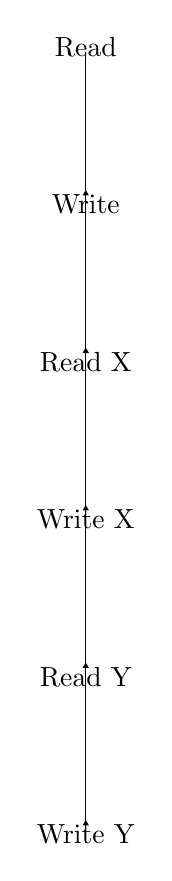
\begin{tikzpicture}[node distance=2cm]
    \node (read) {Read};
    \node [below of=read] (write) {Write};
    \node [below of=write] (readx) {Read X};
    \node [below of=readx] (writex) {Write X};
    \node [below of=writex] (ready) {Read Y};
    \node [below of=ready] (writey) {Write Y};

    % Custom arrow tip style
    \tikzset{
        myarrow/.style={
            -{Triangle[angle=60:1pt 3]},
            shorten >=-5pt,
            shorten <=-5pt,
        }
    }

    % Draw arrows without overlapping content
    \draw [myarrow] (read) -- ++(0,-1) |- (write);
    \draw [myarrow] (write) -- ++(0,-1) |- (readx);
    \draw [myarrow] (readx) -- ++(0,-1) |- (writex);
    \draw [myarrow] (writex) -- ++(0,-1) |- (ready);
    \draw [myarrow] (ready) -- ++(0,-1) |- (writey);

\end{tikzpicture}

\end{document}